\chapter{Physical properties of low temperature RF plasma}

  In this first chapter I will provide the necessary physical background 
  for this work about the numerical simulation of low temperature 
  capacitively coupled radio frequency plasma. Here both the mathematical 
  basics and method for the simulation, as well as the most important aspects
  about the plasma properties will be explained.

  \section{Plasma physics}

    \subsection{Capacitively coupled radio frequency plasma}

      The experiment where after the conducted simulations is modelled after revolves around a capacitively coupled radio frequency, low temperature plasma at low pressures of oxygen. \\
      Here, I will refer to a plasma as an globally quasi-neutral gas, consisting of freely moving charges --- e.g.\@ electrons, positiviely and negatively ions --- and neutral gas particles. The ratio between charged and neutral species defines the \emph{degree of ionization}, which in this case is very low. The term of global neutrality emphasizes the purpose for different lenght scales inside the gas itself. Hence, the associated condition of neutrality by equal densities $n\ix{e}\,=\,n\ix{i}$ only is valid for areas larger than the so called \emph{Debye sphere}. Inside this ball with a radius of $\lambda\ix{D}$, the \emph{Debye length}, the afore-mentioned neutrality is not satisfied.\\
      The creation of a plasma is accomplished by 2 parallel metal plates --- the electrodes --- where on at least one an AC signal at radio frequency is applied --- this kind of experimental setup is among the most common, thus being used for basic but also in-depth studies of the afore-mentioned discharges. Here, a rf signal at exactly $\unit[13,56]{MHz}$ with an amplitude between $100$--$\unit[1000]{V}$ will be used --- this corresponds to a wavelength of $\unit[22,11]{m}$ for the excitation. The use of external magnetic fields is not within the scope of this work --- correspondingly, the experiment I will refer to also did not include $\vec{B}$-fields. \\
      That said, a multitude of electric setups are possible, such as coated or grounded electrodes. Therefore, different regimes of operation ensue. For example, differently driven or shaped metal plates heavily influence the charge creation process inside the plasma. In summary, the electrodes, neutral gas and electric layout resemble a dielectric hindered plate capacitor. This simplification can be used to access important physical properties, such as an additional voltage offset on one of the electrodes or charge currents at such. A basic scheme of an asymmetric rf discharge can be seen in~\autoref{fig:circuitselfbias_1}.

			\begin{wrapfigure}{r}{0.33\textwidth}
				\centering
				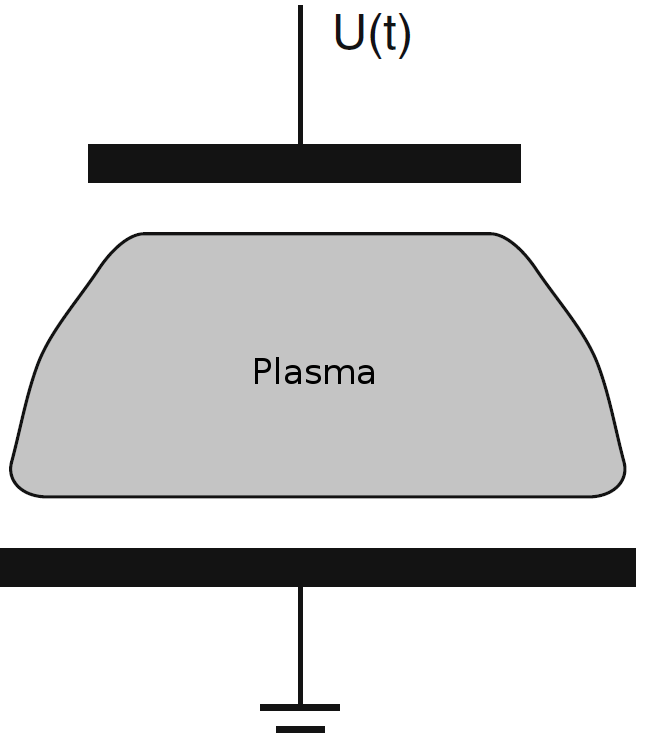
\includegraphics[width=0.3\textwidth,height=0.35\textwidth]{figures/circuitselfbias_1.png}
				\caption{%
				Schematic of an asymmetric discharge with one grounded and one driven electrode.%
				The rf signal is denoted with $U(t)$.}\label{fig:circuitselfbias_1}
			\end{wrapfigure}

      In the case of different electrode sizes, as seen in the scheme, the potential inside the spatially restricted area between wall and discharge can change drastically. This plasma sheath forms also between grounded parts of discharge containment or probes and plasma volume. This additional direct current offset is called \emph{self-bias} (see~\autoref{subsec:selfbias}). A dielectric displacement current between plasma sheath and volume accomodates as a result of the different time scales of particle movement (see~\autoref{subsec:displacementcurrent}). Especially, self-bias and displacement current play a key role in the following investigations, as a capacitive coupling between electrodes and power supply is difficult to model into a numerical kinetic simulation.\\
		In comparison to other low temperature, low pressure discharges  --- an example could be a dielectric hindered dc discharge at high voltages, with an electrode space gap of just a couple millimeters ---, radio frequency plasma are characterized by their unique transport process inside the sheath and heating mechanisms of charged species. A more in-depth discussion can be found in~\autoref{subsec:heating}.\\ 

		\subsection{Sheath physics and wall interaction}\label{subsec:sheathphysics}

		\subsection{Bohm criteria}\label{subsec:bohmcriteria}

			In~\autoref{subsec:sheathphysics} the behaviour of charge particle densities inside the plasma sheath has been discussed. In contrast to the discharge volume, those densities do not satisfy the quasi-neutrality condition in a distance of $d$ from the wall anymore. Though we know that the sheath is a spacially restricted area around electrostatic floating surfaces, a physical law concerning this circumstance has not been derived here. So the question ensues, why the area of electron depletion does not extend further into the discharge volume.\\
		To answer this question, one has to take a look at substitutional system. This will be a, likewise mechanical, one-body extremal problem of a point mass. In this case only kinematic pontentials with inverted parabolic maxima are of interest. Therefore, in this unstable equilibrium a small pertubation culminates into a large force on the test body.\\
		To see the quality of this example, one has to take a look at the second order differential equation of the afore-mentioned mechanical problem and the electrostatic \emph{Poisson's equation} (see~\autoref{equ:pseudo}).

  	\begin{align} 
  	  m\frac{\diff^{2}\vec{r}}{\diff t^{2}}=-\frac{\diff V}{\diff\vec{r}}%
			\quad\Leftrightarrow\quad%
			\Delta_{\vec{r}}\Phi=-\frac{\diff\Psi}{\diff\Phi}=f{\left(\Phi\right)}%
			\hspace{-0.33cm}\overset{\text{Poisson's}}{\overset{\mid}{=}}\hspace{-0.33cm}%
			\frac{\rho}{\varepsilon\ix{0}}\label{equ:pseudo}
  	\end{align}

		For an instability, the force on the test body must increase with the distance from the equilibrium, hence the~\autoref{equ:inequality} is used to calculate the exact velocity at which an ion is entering the sheath. This results in the first \emph{Bohm criteria}.

		\begin{align}
			0>\left.\frac{\diff^{2}\Psi}{\diff\Phi^{2}}\right|_{\Phi=0}%
			\overset{\text{\autoref{equ:pseudo}}}{\overset{\mid}{=}}%
			=\frac{en\ix{e}\left(-d\right)}{\varepsilon\ix{0}}\left(\frac{e}{k\ix{b}T\ix{e}}-\frac{e}{m\ix{i}v\ix{i,0}^{2}}\right)%
			\left.\frac{\diff}{\diff\Phi}\left(\frac{n\ix{e}\left(x\right)-n\ix{i}\left(x\right)}{\varepsilon\ix{0}}\right)\right|_{\Phi=0}&%
			\label{eq:beding} \\%
			\Rightarrow\quad%
			v\ix{i,0}\ge v\ix{i,B}=\sqrt{\frac{k\ix{B}T\ix{e}}{m\ix{i}}}&\label{equ:inequality}
		\end{align}
	
		Analoguos you can define the so called \emph{Mach number} $M=v\ix{i,0}/v\ix{i,B}$, where $v\ix{i,B}$ denotes the \emph{Bohm velocity}.\\
		Now, to understand why the sheath does not extend further than a fixed distance $d$ from the discharge boundary, the particle movement has to be investigated on a smaller scale. As seen above, there is an electric field in the \emph{pre-sheath} that accelerates the ions to $v\ix{i,B}$. In addition, quasi-neutrality is still satisfied here:

		\begin{align}
			n\ix{I}\left(x\right)=n\ix{I,0}\exp\left(\frac{e\Phi\left(x\right)}{k\ix{B}T\ix{e}}\right)%
			=n\ix{e}\left(x\right)\,\,.\label{equ:quasineutral}
		\end{align}

		Still, $\Phi{\left(x\right)}$ is the potential inside the pre-sheath from~\autoref{subsec:sheathphysics} and $n\ix{i,0}$ the unpertubated density from the plasma \emph{bulk}. Though 
		
		\subsection{Self bias voltage}\label{subsec:selfbias}

    \subsection{Dielectric displacement current}\label{subsec:displacementcurrent}

		\subsection{Heating mechanisms}\label{subsec:heating}

  \section{Negative ion physics}

    \subsection{Anion creation and distribution}

    \subsection{Dynamics and collisions}

  \section{Particle-In-Cell simulations with Monte Carlo-Colissions}

    \subsection{Principles}

    \subsection{2d3v PIC}

    \subsection{Monte Carlo-Collisions}
